\section{Foundations: Bandits \& Tabular Methods}

\begin{problem}{Non-Stationary Bandits \& Exponential Moving Average}
Consider a 3-armed bandit problem where the true action values $q_*(a)$ change over time (non-stationary). You are using an $\epsilon$-greedy agent with $\epsilon=0.1$ and a constant step-size parameter $\alpha=0.5$.

At time step $t=1$, the estimated action values are $Q_1(1) = 2.0$, $Q_1(2) = 0.0$, and $Q_1(3) = 1.0$.

The agent selects action $A_1=1$ and receives a reward $R_1=2.0$.
At time step $t=2$, the environment shifts significantly. The true values become $q_*(1)=1.0$, $q_*(2)=5.0$, $q_*(3)=0.0$.
The agent selects action $A_2=2$ and receives a reward $R_2=5.0$.
At time step $t=3$, the agent selects action $A_3=1$ again and receives a reward $R_3=1.0$ (reflecting the new true value).

\begin{enumerate}[label=(\alph*)]
    \item Calculate the updated action-value estimates $Q_2(a)$ after the first step.
    \item Calculate the updated action-value estimates $Q_3(a)$ after the second step.
    \item Calculate the updated action-value estimates $Q_4(a)$ after the third step.
    \item Explain why a constant step-size $\alpha$ is preferred over the sample-average method ($1/n$) in this non-stationary setting.
\end{enumerate}
\end{problem}

\begin{solution}
\textbf{(a) Update after step $t=1$}

The update rule for a constant step-size $\alpha$ is given by:
\[ Q_{k+1}(A_k) = Q_k(A_k) + \alpha [R_k - Q_k(A_k)] \]
where $A_k$ is the action taken and $R_k$ is the reward received.

At $t=1$:
\begin{itemize}
    \item Action $A_1 = 1$.
    \item Reward $R_1 = 2.0$.
    \item Current estimate $Q_1(1) = 2.0$.
    \item $\alpha = 0.5$.
\end{itemize}

Update for action 1:
\[ Q_2(1) = Q_1(1) + 0.5 [2.0 - 2.0] = 2.0 + 0 = 2.0 \]
Estimates for other actions remain unchanged:
\[ Q_2(2) = 0.0, \quad Q_2(3) = 1.0 \]

\textbf{(b) Update after step $t=2$}

At $t=2$:
\begin{itemize}
    \item Action $A_2 = 2$.
    \item Reward $R_2 = 5.0$.
    \item Current estimate $Q_2(2) = 0.0$.
\end{itemize}

Update for action 2:
\[ Q_3(2) = Q_2(2) + 0.5 [5.0 - 0.0] = 0.0 + 2.5 = 2.5 \]
Estimates for other actions remain unchanged:
\[ Q_3(1) = 2.0, \quad Q_3(3) = 1.0 \]

\textbf{(c) Update after step $t=3$}

At $t=3$:
\begin{itemize}
    \item Action $A_3 = 1$.
    \item Reward $R_3 = 1.0$ (reflecting the new true value).
    \item Current estimate $Q_3(1) = 2.0$.
\end{itemize}

Update for action 1:
\[ Q_4(1) = Q_3(1) + 0.5 [1.0 - 2.0] = 2.0 + 0.5(-1.0) = 2.0 - 0.5 = 1.5 \]
Estimates for other actions remain unchanged:
\[ Q_4(2) = 2.5, \quad Q_4(3) = 1.0 \]

Final Estimates $Q_4$:
\[ Q_4(1) = 1.5, \quad Q_4(2) = 2.5, \quad Q_4(3) = 1.0 \]

\textbf{(d) Constant Step-size vs Sample Average}

Using a constant step-size $\alpha \in (0, 1]$ results in an exponentially weighted moving average (EWMA). Recent rewards are given more weight than older rewards.
\[ Q_{k+1} = (1-\alpha)^k Q_1 + \sum_{i=1}^{k} \alpha(1-\alpha)^{k-i} R_i \]
In a non-stationary environment, old rewards become irrelevant as the true values change. The sample-average method ($1/n$) treats all rewards equally (weight $1/k$ for the $k$-th reward decreases to 0), meaning the agent's estimate will lag significantly behind the changing true value and may never converge to the new value if $n$ is large. A constant $\alpha$ ensures the agent remains responsive to recent changes.
\end{solution}

\newpage

\begin{problem}{SARSA vs Q-Learning in Grid World}
Consider the following 3x3 Grid World.
\begin{center}
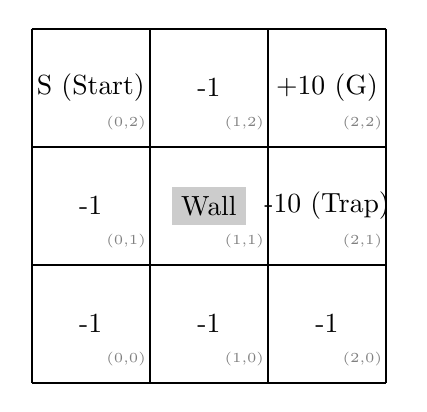
\begin{tikzpicture}[scale=1.5]
    \draw[thick] (0,0) grid (3,3);

    % States
    \node at (0.5, 2.5) {S (Start)};
    \node at (1.5, 2.5) {-1};
    \node at (2.5, 2.5) {+10 (G)};

    \node at (0.5, 1.5) {-1};
    \node[fill=black!20] at (1.5, 1.5) {Wall};
    \node at (2.5, 1.5) {-10 (Trap)};

    \node at (0.5, 0.5) {-1};
    \node at (1.5, 0.5) {-1};
    \node at (2.5, 0.5) {-1};

    % Coordinates labels
    \foreach \x in {0,1,2} \foreach \y in {0,1,2} \node[font=\tiny, gray] at (\x+0.8, \y+0.2) {(\x,\y)};
\end{tikzpicture}
\end{center}
States are denoted by $(x,y)$ where $x$ is column index (0-2) and $y$ is row index (0-2).
Start state $S$ is at $(0,2)$. Goal state $G$ is at $(2,2)$ with reward $+10$ (terminal).
The "Trap" at $(2,1)$ gives reward $-10$. All other transitions give reward $R=-1$.
Actions: Up, Down, Left, Right.
Assume $\gamma = 0.9$ and $\alpha = 0.5$.
Initial Q-values $Q(s,a) = 0$ for all states and actions.

Consider the following episode trajectory:
1. Start at $S(0,2)$. Agent chooses \textbf{Right}.
2. Lands in $(1,2)$, receives $R=-1$. From $(1,2)$, the agent's policy (e.g., $\epsilon$-greedy) chooses \textbf{Right} again.
3. However, before the update, we need to consider the algorithm.

\textbf{Scenario:}
The agent is at $S(0,2)$, takes action $A=$ Right, lands in $S'=(1,2)$, receives $R=-1$.
The agent then chooses the next action $A'$ from $S'$.
Suppose the greedy action at $S'$ is \textbf{Right} (towards Goal), but the exploratory action chosen is \textbf{Down} (towards Wall, stays in place or bounces).
Let's simplify:
\begin{itemize}
    \item $S = (0,2)$
    \item $A = \text{Right}$
    \item $R = -1$
    \item $S' = (1,2)$
    \item Greedy action at $S'$: $a^* = \text{Right}$ (leads to Goal, hypothetically best).
    \item Actual next action chosen $A' = \text{Down}$ (leads to Wall/Collision).
\end{itemize}

Note: For this problem, assume Q-values are initialized to 0. If multiple actions have max Q-value, ties are broken arbitrarily (say, Up $>$ Right $>$ Down $>$ Left).
Since all Q=0, $Q(S', \text{Right}) = 0$ and $Q(S', \text{Down}) = 0$.
So initially, the values don't distinguish.

Let's assume a pre-trained table where some values are learned to make the difference clear.
Suppose at $S'=(1,2)$:
\begin{itemize}
    \item $Q(S', \text{Right}) = 5.0$ (Learned path to goal)
    \item $Q(S', \text{Down}) = -2.0$ (Learned path to nowhere)
\end{itemize}
And at $S=(0,2)$, $Q(S, \text{Right}) = 1.0$.

\textbf{Task:}
Using the transition $S \xrightarrow{A=\text{Right}} S' (R=-1)$ and the next chosen action $A'=\text{Down}$:
\begin{enumerate}[label=(\alph*)]
    \item Calculate the updated $Q(S, \text{Right})$ using the \textbf{SARSA} update rule.
    \item Calculate the updated $Q(S, \text{Right})$ using the \textbf{Q-Learning} update rule.
    \item Explain the significance of the difference in these values in the context of "On-Policy" vs "Off-Policy" learning.
\end{enumerate}
\end{problem}

\begin{solution}
\textbf{Given Parameters:}
\begin{itemize}
    \item $\alpha = 0.5$, $\gamma = 0.9$
    \item Transition: $S=(0,2) \xrightarrow{\text{Right}} S'=(1,2)$, $R=-1$.
    \item Current Q-value: $Q(S, \text{Right}) = 1.0$.
    \item At $S'$, values are: $Q(S', \text{Right}) = 5.0$, $Q(S', \text{Down}) = -2.0$.
    \item Next actual action chosen: $A' = \text{Down}$.
\end{itemize}

\textbf{(a) SARSA Update}
SARSA (State-Action-Reward-State-Action) is an \textbf{On-Policy} algorithm. It updates the Q-value based on the action actually taken by the current policy ($A'$).
\[ Q(S, A) \leftarrow Q(S, A) + \alpha [ R + \gamma Q(S', A') - Q(S, A) ] \]

Substitute the values:
\begin{itemize}
    \item $Q(S', A') = Q(S', \text{Down}) = -2.0$.
\end{itemize}
\[ Q(S, \text{Right}) \leftarrow 1.0 + 0.5 [ -1 + 0.9(-2.0) - 1.0 ] \]
\[ Q(S, \text{Right}) \leftarrow 1.0 + 0.5 [ -1 - 1.8 - 1.0 ] \]
\[ Q(S, \text{Right}) \leftarrow 1.0 + 0.5 [ -3.8 ] \]
\[ Q(S, \text{Right}) \leftarrow 1.0 - 1.9 = -0.9 \]

The value decreased significantly because the agent actually took a bad action (Down) in the next state.

\textbf{(b) Q-Learning Update}
Q-Learning is an \textbf{Off-Policy} algorithm. It updates the Q-value based on the best possible action in the next state (Greedy), regardless of what action the agent actually takes.
\[ Q(S, A) \leftarrow Q(S, A) + \alpha [ R + \gamma \max_{a} Q(S', a) - Q(S, A) ] \]

Substitute the values:
\begin{itemize}
    \item $\max_{a} Q(S', a) = \max(Q(S', \text{Right}), Q(S', \text{Down}), \dots) = \max(5.0, -2.0) = 5.0$.
\end{itemize}
\[ Q(S, \text{Right}) \leftarrow 1.0 + 0.5 [ -1 + 0.9(5.0) - 1.0 ] \]
\[ Q(S, \text{Right}) \leftarrow 1.0 + 0.5 [ -1 + 4.5 - 1.0 ] \]
\[ Q(S, \text{Right}) \leftarrow 1.0 + 0.5 [ 2.5 ] \]
\[ Q(S, \text{Right}) \leftarrow 1.0 + 1.25 = 2.25 \]

The value increased because Q-Learning assumes the agent will act optimally from the next state onwards, ignoring the exploratory "mistake" (Down).

\textbf{(c) Significance}
The difference highlights the distinction between On-Policy and Off-Policy learning:
\begin{itemize}
    \item **SARSA** learns the value of the \textit{actual policy} being followed, including its exploration steps (epsilon-greedy). If the policy explores often (high epsilon) and takes dangerous actions (like 'Down' into a trap or wall), SARSA will propagate that risk back, lowering the Q-value of the previous state. It learns a "safer" path.
    \item **Q-Learning** learns the value of the \textit{optimal policy}, assuming that exploration is just a temporary anomaly. It is more aggressive/optimistic, learning the shortest path along the cliff edge because it assumes optimal behavior in the future, even if the current policy is likely to fall off.
\end{itemize}
\end{solution}

\newpage
